\documentclass[tikz,border=6pt]{standalone}
\usepackage{amsmath}
\usepackage{helvet}
\usepackage{xcolor}
\renewcommand{\familydefault}{\sfdefault}
\usetikzlibrary{arrows.meta,positioning,calc}

\definecolor{myblue}{HTML}{377EB8}
\definecolor{myred}{HTML}{E41A1C}
\definecolor{myviolet}{HTML}{984EA3}

\begin{document}

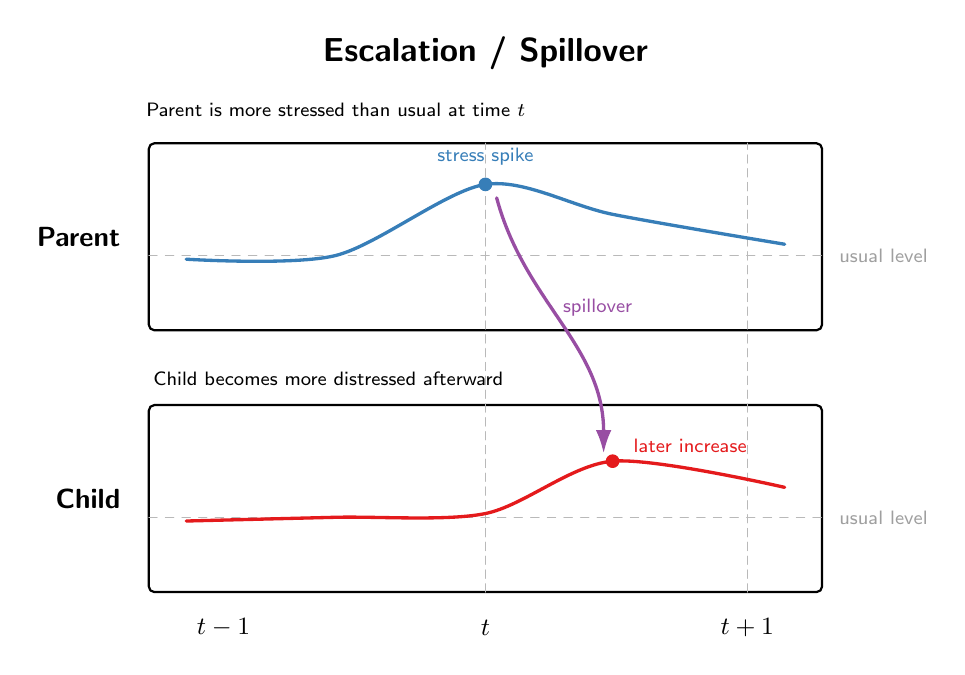
\begin{tikzpicture}[
		x=0.95cm,
		y=0.95cm,
		>=Latex,
		line cap=round,
		line join=round,
		eventdot1/.style={circle,fill=myblue,draw=myblue,inner sep=1.6pt},
		eventdot2/.style={circle,fill=myred,draw=myred,inner sep=1.6pt},
		note/.style={font=\scriptsize,align=center},
		paneltitle/.style={font=\bfseries},
		guide/.style={densely dashed,gray!55},
		baseline/.style={dashed,gray!55},
		flow/.style={-{Latex[length=3mm,width=2mm]},very thick,draw=myviolet}
	]
	
	% Coordinates for shared times
	\coordinate (tm1) at (1,0);
	\coordinate (tt)  at (4.5,0);
	\coordinate (tp1) at (8,0);
	
	% Main title
	\node[font=\bfseries\large] at (4.5,7.9) {Escalation / Spillover};
	
	% Panel boxes
	\draw[thick,rounded corners=2pt] (0,4.2) rectangle (9,6.7);
	\draw[thick,rounded corners=2pt] (0,0.7) rectangle (9,3.2);
	
	% Panel labels
	\node[anchor=east,paneltitle] at (-0.25,5.45) {Parent};
	\node[anchor=east,paneltitle] at (-0.25,1.95) {Child};
	
	% Usual levels
	\draw[baseline] (0,5.2) -- (9,5.2);
	\draw[baseline] (0,1.7) -- (9,1.7);
	
	\node[anchor=west,font=\scriptsize,gray!75] at (9.1,5.2) {usual level};
	\node[anchor=west,font=\scriptsize,gray!75] at (9.1,1.7) {usual level};
	
	% Vertical time guides
	\draw[guide] (4.5,0.7) -- (4.5,6.7);
	\draw[guide] (8,0.7) -- (8,6.7);
	
	% Time labels
	\node[font=\small] at (1,0.22) {$t-1$};
	\node[font=\small] at (4.5,0.22) {$t$};
	\node[font=\small] at (8,0.22) {$t+1$};
	
	% Parent trajectory
	\draw[very thick,myblue]
	plot[smooth] coordinates {
		(0.5,5.15)
		(2.5,5.2)
		(4.5,6.15)
		(6.2,5.75)
		(8.5,5.35)
	};
	
	% Child trajectory
	\draw[very thick,myred]
	plot[smooth] coordinates {
		(0.5,1.65)
		(2.5,1.7)
		(4.5,1.75)
		(6.2,2.45)
		(8.5,2.1)
	};
	
	% Key event dots
	\node[eventdot1] (parentpeak) at (4.5,6.15) {};
	\node[eventdot2] (childrise)  at (6.2,2.45) {};
	
	% Short local annotations
	\node[note,anchor=south,text=myblue] at (4.5,6.28)
	{stress spike};
	\node[note,anchor=west,text=myred] at (6.35,2.66)
	{later increase};
	
	% Cross-panel arrow showing spillover
	\draw[flow] ($(parentpeak)+(0.15,-0.18)$) to[out=-75,in=90] ($(childrise)+(-0.12,0.10)$);
	
	\node[note,text=myviolet] at (6.0,4.50) {spillover};
	
	% Explanatory captions
	\node[note] at (2.5,7.15)
	{Parent is more stressed than usual at time $t$};
	
	\node[note] at (2.4,3.55)
	{Child becomes more distressed afterward};
	
\end{tikzpicture}

\end{document}
